\section{Protocol to assign map sampling rate and origin of coordinates}
\label{app:asignOrigAndSampling}%a161

Protocol designed to modify the values of sampling rate and origin of coordinates of electron density maps that are already in the \scipion workflow. Remark that the new map generated in the \scipion workflow will associate these two attributes, samplig rate and origin of coordinates, WITHOUT modifying the map header. If you want to modify the map header inside \scipion, for example to deposit it to EMDB, you should use the protocol \scommand{export to DB}.
   
 \begin{itemize}
  \item Requirements to run this protocol and visualize results:
    \begin{itemize}
        \item \scipion plugin: \ttt{scipion-em}
    \end{itemize}
  \item \scipion menu:
  It does not appear in \ttt{Model building} view.
  Press \scommand{Ctrl} + \scommand{f} and the pop up window to search a protocol will be opened ((\ffigure{fig:app_protocol_assign_orig_and_sampling} (A)). Write any word related with the title of the protocol that you are looking for in the \ttt{Search} box. In this particular case we have written \ttt{origin}. Several protocols have been found related with this search word. Select the third one dessigned for the purpose that we are interested in (\ttt{pwem - assign orig \& sampling}).
  
    \begin{figure}[H]
    \centering 
    \captionsetup{width=.7\linewidth} 
    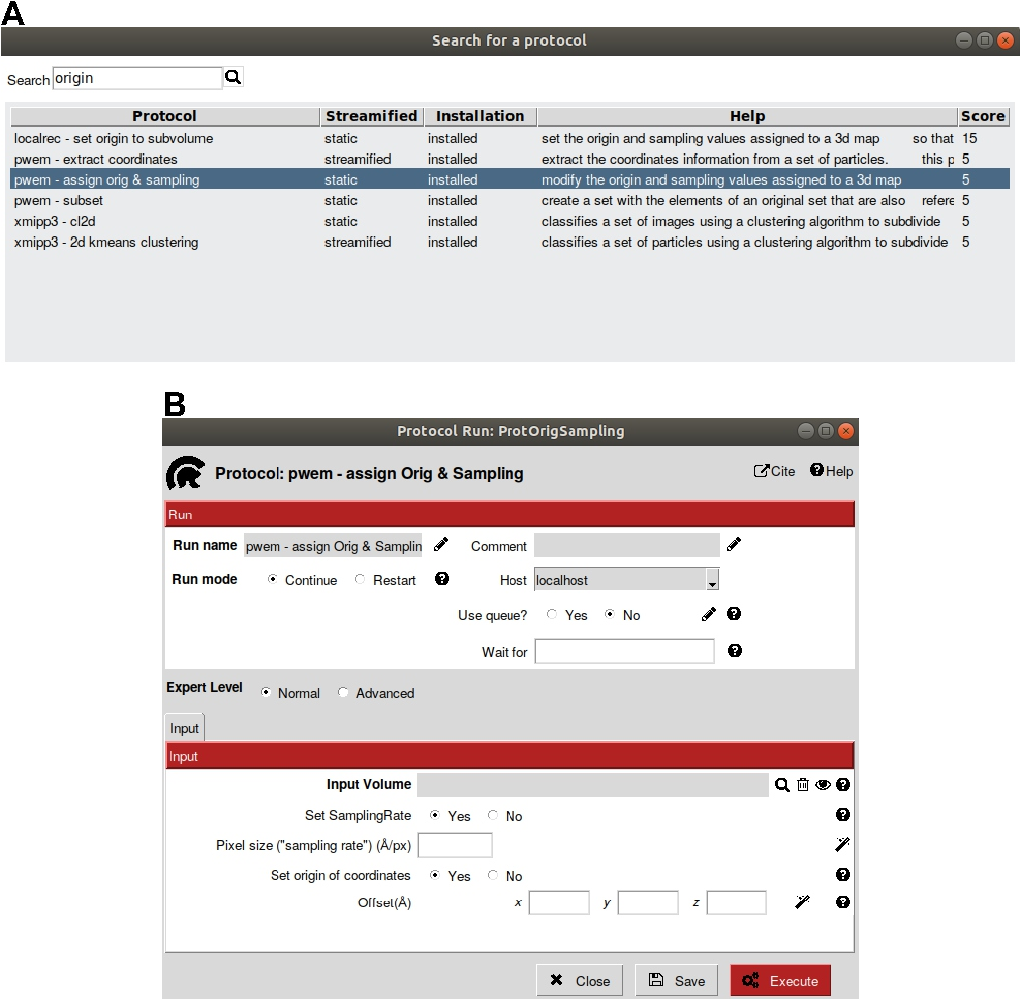
\includegraphics[width=0.90\textwidth]{Images_appendix/Fig301.pdf}
    \caption{A. Protocol \scommand{assign Orig \& Sampling}. A: Window to search the protocol. B: Protocol form.}
    \label{fig:app_protocol_assign_orig_and_sampling}
   \end{figure}
  
  \item Protocol form parameters (\ffigure{fig:app_protocol_assign_orig_and_sampling} (B)):
  
  \begin{itemize}
   \item \ttt{Input} section
  

  \begin{itemize}
   \item \ttt{Input Volume}: Include here any map previously downloaded or generated in \scipion that you would like to assing a new sampling rate and/or origin of coordinates.
   \item \ttt{Set SamplingRate)}: Select \ttt{Yes} if you want to give the map a new value of sampling rate. Then, a new form box will appear:
    \begin{itemize}
    \item \ttt{Pixel size (``sampling rate'')} (\AA/px): Write the new sampling rate rate value in the box. Remark that you have a wizard on the right to check the current value.
    \end{itemize}
   \item \ttt{Set origin of coordinates}: You have to choose between setting the previously origin of coordinates assigned in \scipion (option ``No'') or another origin of coordinates (``Yes''). If you decide to set your own origin of coordinates (option ``Yes''), a new form parameter (\ttt{Offset}) will appear below.
    \begin{itemize}
   \item \ttt{Offset}: Write here x, y, and z coordinates of your preference (in \AA). As in the case of the \ttt{Pixel size}, remark that you have a wizard on the right side of the parameter to check the header current coordinates of the origin. 
    \end{itemize}
   \end{itemize}
   
  
  \end{itemize}
  \item Protocol execution:
  
  Adding specific volume label is recommended in \ttt{Run name} section, at the form top. To add the label, open the protocol form, press the pencil symbol at the right side of \ttt{Run name} box, complete the label in the new opened window, press OK, and finally, close the protocol. This label will be shown in the output summary content (see below). If you want to run again this protocol, do not forget to set to \ttt{Restart} the \ttt{Run mode}.\\
  Press the \ttt{Execute} red button at the form bottom.
  
  \item Visualization of protocol results:
  
  After executing the protocol, press \ttt{Analyze Results} and $ShowJ$, the default \scipion viewer, will allow you to visualize the \ttt{slices} window of the map  (\ffigure{fig:app_protocol_assign_orig_and_sampling_2}). The $ShowJ$ window menu (\ttt{File -> Open with ChimeraX}) allows to open the selected map in $ChimeraX$ graphics window.
   
   \begin{itemize}
  \item \ttt{slices}: $ShowJ$
   
\url{https://github.com/I2PC/scipion/wiki/ShowJ}


   \begin{figure}[H]
   \centering 
    \captionsetup{width=.7\linewidth} 
    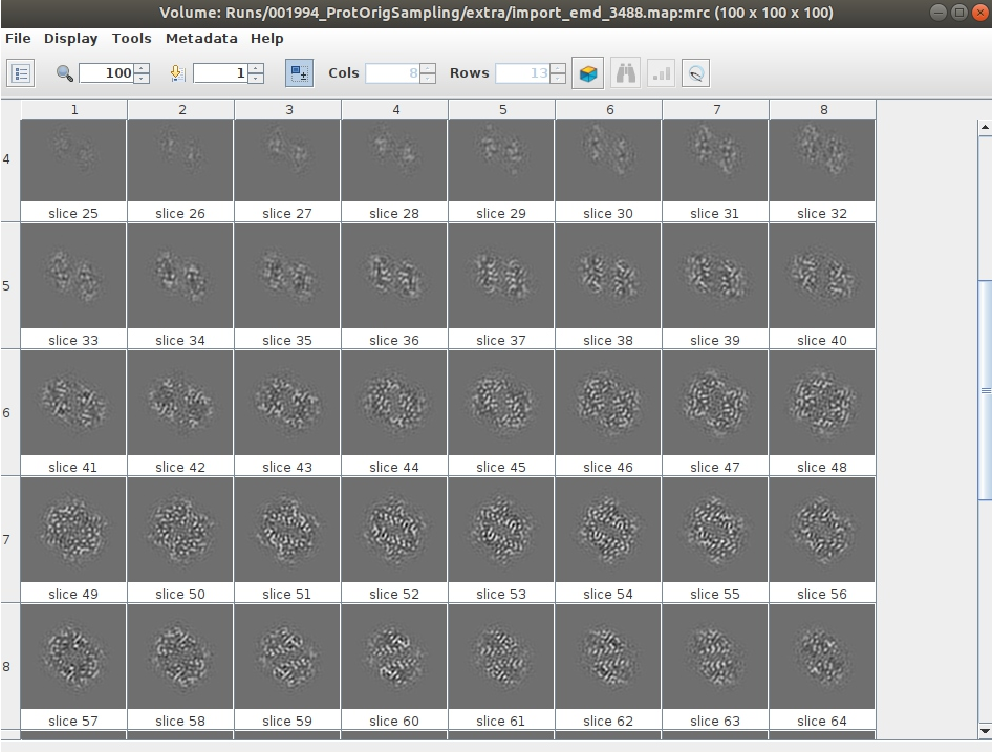
\includegraphics[width=0.75\textwidth]{Images_appendix/Fig302.pdf}
    \caption{Protocol \scommand{assign Orig \& Sampling}. Gallery model of $ShowJ$ to visualize the map slices.}
    \label{fig:app_protocol_assign_orig_and_sampling_2}
   \end{figure}
   
   \end{itemize}
   
   \item Summary content:
    
    \begin{itemize}
     \item Protocol output (below \scipion framework):\\ \ttt{pwem - assign Orig \& Sampling -> ouputVolume};\\ \ttt{Volume (x, y, and z dimensions, NEW sampling rate)}.
     \item \ttt{SUMMARY} box:\\\ttt{New Sampling}: New assigned value of sampling rate.\\\ttt{New Origin}: Coordinates \ttt{x, y, z} of the new assigned origin of coordinates.
    \end{itemize}
  
  \end{itemize}
